\fancyhf{}
\pagestyle{fancy}
%Encabezado
\lhead[]{\leftmark}
\chead[]{}
\rhead[]{\thepage}
\renewcommand{\headrulewidth}{1pt}

\section{Introducción}

En el capítulo anterior, se explicó la importancia de analizar identificadores (ids) ubicados en el código fuente de un sistema de software. Los ids de un programa normalmente están compuestos por más de una palabra en forma de abreviatura, por ejemplo: \textsf{inp\_fl\_sys}. Detrás de estas abreviaturas, los ids ocultan información es propia del Dominio del Problema \cite{BCPT99,LFBEX07,EZH08,EHPV09}. Desafortunadamente, las personas ajenas al código, no comprenden a simple vista la información que los ids poseen en sus abreviaturas e invierten tiempo en entenderlas. Es por esto, que las herramientas automáticas de análisis de ids son bienvenidas en el ámbito de la Comprensión de Programas (CP). Con estas herramientas se logra disminuir los tiempos de comprensión de ids y revelar la información que estos contienen en sus abreviaturas.

Dada la importancia que tienen las herramientas de análisis de ids, se tomó la iniciativa de desarrollar una llamada Identifier Analyzer (IDA). Esta herramienta le permite al usuario ingresar un archivo JAVA, luego IDA analiza los ids que están en el archivo.
%, y finalmente produce como resultado una tabla del análisis realizado, esta tabla contiene los ids encontrados en el programa pero expandidos. 
IDA lleva a cabo el análisis de ids en tres pasos, los cuales se mencionan a continuación: I) Extraer los ids del código de estudio. II) Aplicar una técnica de división, en donde se descomponen a los ids en las distintas abreviaturas que lo componen. Por ejemplo: \textsf{inp\_fl\_sys} $\Rightarrow$ \textsf{inp fl sys}. III) Emplear una técnica de expansión de abreviaturas que las expande a palabras completas. Por ejemplo: \textsf{inp fl sys} $\Rightarrow$ \textsf{input file system}. Una vez realizado los tres pasos, los resultados de las expansiones de ids se exhiben en una tabla.
El objetivo de IDA es lograr que el usuario comprenda más rápidamente el propósito de los ids en los archivos JAVA, y de esta manera mejorar la comprensión del código analizado.

%Para que IDA pueda realizar su tarea, contiene implementados 2 algoritmos de división de ids (Greedy y Samurai) y 1 algoritmo de expansión de abreviaturas (Expansión Básica), los mismos fueron explicados en el capítulo precedente. 

El correspondiente capítulo, está destinado a explicar los distintos módulos que IDA posee, y que proceso de ejecución debe realizar el usuario para analizar los ids.
Para comenzar con la descripción de IDA, en la siguiente sección se explica la arquitectura y cuales son sus componentes principales.

%La herramienta IDA le permite al usuario ingresar archivos con código JAVA. Luego la herramienta ejecuta técnicas/algoritmos que analizan los ids situados en el código del archivo.

%La herramienta IDA le permite al usuario revelar la información estática oculta que hay detrás de los ids. Esto se logra mediante la ejecución de técnicas/algoritmos que fueron descriptos en el capítulo anterior.
%
%La iniciativa del desarrollo de la herramienta IDA surgió, porque en la actualidad no existe otra herramienta en el ámbito de la CP con similares características.

%El objetivo de aplicar estas técnicas consiste en convertir los ids que están abreviados a palabras completas más entendibles para el lector ajeno al código.

%Una vez realizada esta conversión, IDA le permite al usuario reemplazar a elección los ids con los nuevos nombres, creando así un nuevo archivo con código más legible y sin alterar la funcionalidad original del código. 

\begin{figure}[t] %[h] para here [b] para bottom [t] para top
\centerline{%queda centrada mejor la imagen
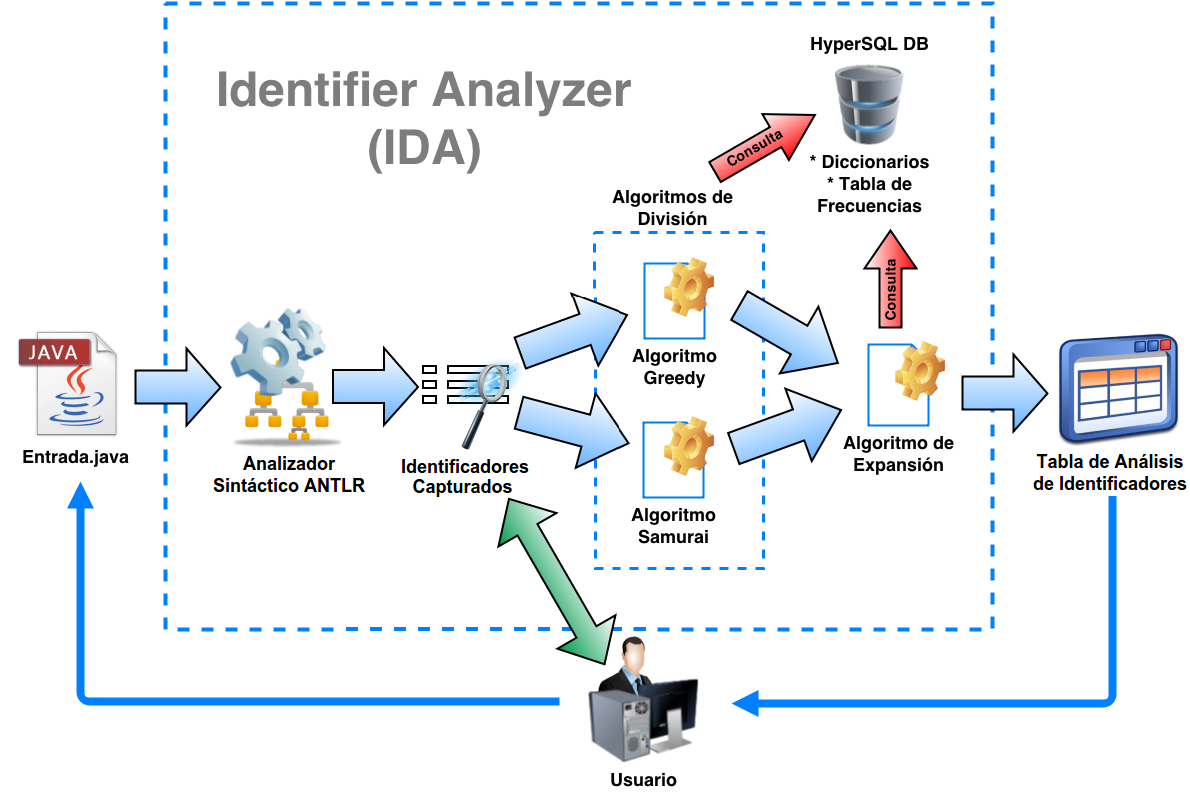
\includegraphics[scale= 0.35]{./cap4/ida_arq.png}
}
\caption{Arquitectura de IDA}
\label{arq1}
\end{figure}


\section{Arquitectura}

%La herramienta IDA se implementó empleando lenguaje JAVA y se programó usando el entorno de desarrollo NetBeans\footnote[1]{https://www.netbeans.org}. 

En la Figura \ref{arq1} se puede apreciar la arquitectura de IDA. Esta arquitectura describe tres partes principales, la primera consiste en la \textit{extracción de datos}, la segunda trata sobre la \textit{división de ids} y la tercera sobre \textit{expansión de ids}. A continuación se detallan cada una de ellas.\\

\textbf{Módulo de Extracción de Datos:} Este módulo recibe como entrada un archivo JAVA que ingresa el usuario (Ver Figura \ref{arq1} Entrada.java), luego este archivo se procesa por un Analizador Sintáctico (AS) (\mbox{Ver Figura \ref{arq1}} Analizado Sintáctico ANTLR). El AS, extrae y almacena, en estructuras internas, la información estática perteneciente al código del archivo ingresado. Esta información, está relacionada con ids, literales y comentarios (Ver próxima sección para más detalles). El usuario a través de la interfaz de IDA, puede visualizar esta información capturada del código por medio de tablas claramente definidas (Ver Figura \ref{arq1} - Flecha Verde).

\textbf{Módulo de División de Ids:} Una vez completada la extracción de información, el proceso continua en el módulo de división de ids. Aquí se encuentran implementados dos algoritmos de división; uno es el Algoritmo Greedy y el otro es el Algoritmo Samurai ambos explicados en la sección \ref{sec:algGre} y \ref{sec:algSamu} del capítulo anterior. Estos algoritmos reciben como entrada la información capturada en el módulo de extracción de datos (ids, comentarios, literales), y luego estos algoritmos dividen los ids del archivo JAVA (Ver Figura \ref{arq1} - Algoritmos de División). Los resultados de las divisiones se almacenan en estructuras internas que serán utilizadas por el módulo de expansión. Cabe recordar que estos algoritmos de división necesitan datos externos para funcionar, uno es el diccionario de palabras (en caso de Greedy) y el otro es lista de frecuencias globales de aparición de palabras (en caso de Samurai). Estos datos externos se encuentran almacenados en una base de datos embebida (Ver Figura \ref{arq1} - HyperSQL DB).

\textbf{Módulo de Expansión de Ids:} La tercera y última parte, tiene implementado el Algoritmo de Expansión Básico de abreviaturas que fue explicado en la sección \ref{sec:algExpBas} del capítulo anterior.
Este algoritmo, toma como entrada los ids separados en el módulo de división de ids (tanto de Greedy como de Samurai), luego el Algoritmo de Expansión expande las abreviaturas resultantes producto de la división de ids (Ver Figura \ref{arq1} - Algoritmo de Expansión). Los resultados de las expansiones se retornan en dos grupos: las expansiones provistas por el Algoritmo de división Greedy y las provistas por el Algoritmo de división Samurai.

%En este punto, el usuario podrá elegir que expansión es la más adecuada y reemplazar los ids originales en el archivo de entrada, generando de esta manera un nuevo archivo de salida (ver figura \ref{arq1} Salida.java). 

El \mbox{Algoritmo} de Expansión también necesita de un diccionario de palabras, por eso se realizan consultas a la base de datos embebida (Ver Figura \ref{arq1} - HyperSQL DB). Finalmente, los resultados de las divisiones y las expansiones de los ids, se muestran en una tabla (Ver Figura \ref{arq1} - Tabla de análisis de identificadores).

\section{Analizador Sintáctico}

Como se explicó en la sección previa, cuando el usuario ingresa un archivo JAVA, IDA examina y extrae información estática presente en el archivo ingresado. Esta información está compuesta por identificadores, comentarios y literales. La manera en que IDA extrae esta información es a través de un Analizador Sintáctico (AS).

La construcción de este AS se llevó a cabo, primero investigando herramientas encargadas de construir AS. Se dio preferencia a aquellas que emplean la teoría asociada a las gramáticas de atributos \cite{AHUL06}. De la investigación previamente descripta, se determinó que la herramienta \textit{ANTLR}\footnote[1]{ANother Tool for Language Recognition. http://www.antlr.org} era la que mejor se ajustaba a las necesidades antes planteadas. 
Esta herramienta permite agregar acciones semánticas (escritas en JAVA) para el cálculo de los atributos, en una gramática de lenguaje JAVA\footnote[2]{http://docs.oracle.com/javase/specs/jls/se7/jls7.pdf}. Estas acciones semánticas deben estar correctamente insertadas en la gramática para, por ejemplo, implementar estructuras de datos y algoritmos que capturan los ids utilizados en un programa \cite{AAJU83}. Una vez insertadas estas acciones, ANTLR lee la gramática y genera el AS adicionando acciones que fueron programadas. De esta manera, se obtiene un AS que recolecta ids mientras examina el código. A su vez a estas acciones semánticas, se le agregan otras acciones que extraen comentarios y literales strings. Estos elementos son necesarios ya que sirven para los algoritmos de análisis de ids que serán explicados en próximas secciones.

\section{Base de Datos Embebida}
\label{sec:bseEmb}

Como se describió en secciones previas, IDA posee una base de datos embebida. Esta base de datos utiliza una tecnología llamada HSQLDB\footnote[1]{Hyper SQL Data Base. http://www.hsqldb.org}. Dado que HSQLDB esta desarrollada en JAVA, al momento de incorporarla en IDA (que está programada en JAVA) no resulto una tarea difícil.
Otra ventaja por la cual se eligió esta tecnología, es que responde rápidamente las consultas. Esto es importante ya que todos los algoritmos de IDA consultan a HSQLDB. Dentro de esta base de datos embebida, se encuentran almacenadas los diccionarios/listas de palabras que IDA necesita para llevar adelante sus tareas. Estos diccionarios/listas se describen a continuación, nombrando también que algoritmo de IDA consulta cada diccionarios/listas.

\begin{description}
\itemsep0em%reduce espacio

\item[Diccionario en Inglés (ispell):] Contiene palabras en Inglés que pertenecen a la lista de Palabras Comando de Linux \textit{Ispell}\footnote[2]{ http://wordlist.aspell.net}. Se utiliza en el Algoritmo de Greedy y en el Algoritmo de Expansión (Ver Capítulo 3).

\item[Lista de Palabras Excluyentes (stop-list):] Esta compuesta con palabras que son poco importantes o irrelevantes en el análisis de ids\footnote[3]{ http://www.lextek.com/manuals/onix/stopwords1.html}. Se utiliza en el Algoritmo de Greedy y en el Algoritmo de Expansión \mbox{(Ver Capítulo 3)}.

\item[Lista de Abreviaturas y Acrónimos Conocidas:] Contiene abreviaturas comunes del idioma Inglés y Acrónimos conocidos de programación\footnote[4]{http://langs.eserver.org/acronym-dictionary.txt} (gif, jpg, txt). Se emplea en el Algoritmo Greedy (Ver Capítulo 3).
\pagebreak
\item[Lista de Prefijos y Sufijos Conocidos:] Posee Sufijos y Prefijos conocidos en Inglés\footnote[1]{http://www.eecis.udel.edu/˜enslen/Site/Samurai}, esta lista fue confeccionada por el autor del Algoritmo Samurai (Ver Capítulo 3). Se consulta solo en dicho algoritmo.

\item[Frecuencias Globales de Palabras:] Lista de palabras, junto con su frecuencia de aparición. Esta lista fue construida por el autor del Algoritmo Samurai\footnote[2]{Esta lista no está disponible en la web, por ende se construyó una aproximación.}. Se emplea solo en dicho algoritmo, más precisamente en la función de \textit{Scoring} (Ver Capítulo 3).

\end{description}

Cabe destacar que las listas y diccionarios que fueron descriptos poseen palabras que pertenecen al idioma Inglés, dado que los autores así lo determinaron. Por lo tanto, para que la herramienta IDA analice correctamente los ids, se deben ingresar en IDA archivos JAVA con comentarios, literales e ids acordes a la lengua Inglesa.\\ 

Habiendo descripto los principales módulos de la herramienta, en la próxima sección se explicará el proceso que debe seguir el usuario para analizar ids a través de IDA.
 
\section{Proceso de Análisis de Identificadores}

En esta sección, se describe el proceso que debe seguir el usuario con la herramienta IDA para llevar a cabo el análisis de los ids, en los archivos JAVA. Se explicará que función cumple cada elemento de IDA (ventanas, botones, paneles, etc.), y de como estos elementos ayudan al usuario a analizar los ids.

\subsection{Barra de Menú}

Al ejecutar la herramienta IDA, el primer componente de interacción es una simple barra de menú ubicada en el tope de la pantalla, los botones de esta barra son \textit{Archivo}, \textit{Diccionarios} y \textit{Ayuda} (Ver Figura \ref{ida1}). 

\begin{figure}[t] %[h] para here [b] para bottom [t] para top
\centerline{%queda centrada mejor la imagen
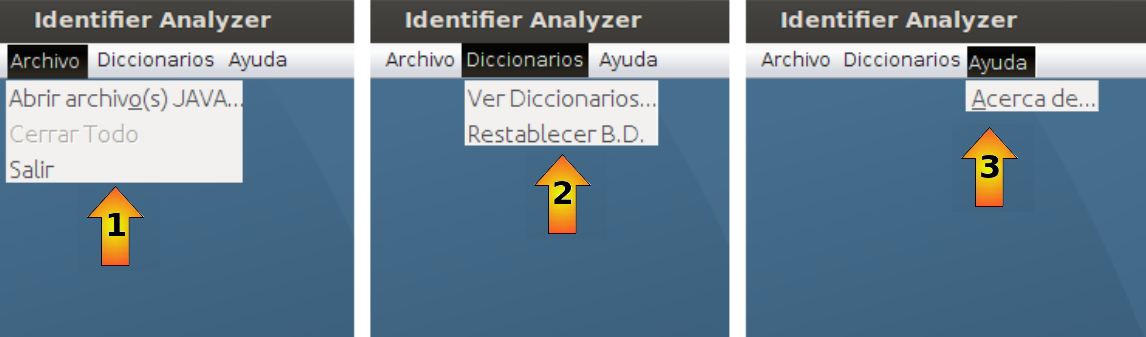
\includegraphics[scale= 0.46]{./cap4/ida_01.png}
}
\caption{Barra de Menú de IDA}
\label{ida1}
\end{figure}

Al pulsar\footnote[1]{El término `pulsar' o `presionar' se utilizará a lo largo del capítulo, significa hacer click con el puntero del ratón.} en \textit{Archivo} de la barra antedicha, se despliega un menú con las opciones que se describen a continuación (Ver Figura \ref{ida1} - Flecha 1):

\begin{description}
\itemsep0em%reduce espacio
\item[Abrir archivo(s) JAVA:] Abre una ventana que permite elegir uno o varios archivos con extensión JAVA (Ver Figura \ref{ida2}). Los archivos seleccionados serán analizados por IDA (en la próxima sección, serán dados más detalles).
\item[Cerrar Todo:] Cierra todos los archivos JAVA abiertos actualmente en la aplicación.
\item[Salir:] Cierra la Aplicación.
\end{description}

Cuando se pulsa en \textit{Diccionarios} de la barra de menú, se despliega otro menú con las siguientes opciones (Ver Figura \ref{ida1} - Flecha 2):

\begin{description}
\itemsep0em%reduce espacio

\item[Ver Diccionarios:] Abre una ventana, que muestra un listado de palabras en Inglés correspondiente al diccionario \textit{ispell} (explicado en la sección anterior). %\footnote[1]{Comando de Linux generalmente utilizado para corregir errores ortográficos (inglés) en archivos de texto. http://wordlist.aspell.net}. 
La ventana antedicha, también muestra un listado de palabras irrelevantes o stoplist (explicado en la sección anterior). Esta ventana, se explica con más detalles en la sección \ref{sec:panPalDicc}.

\item[Restablecer B.D.(Base de Datos):] Genera nuevamente la base de datos HSQLDB. En caso de haber problemas con la base de datos, es útil restablecerla.

%Esta regeneración toma datos de los archivos ubicados en la carpeta `Diccionarios' dentro del proyecto de la herramienta IDA. Restablecer la base es útil cuando se agregan nuevos datos a los diccionarios desde los archivos previamente descriptos.
\end{description}

Finalmente al presionar \textit{Ayuda} de la barra de menú, se despliega un solo botón, el cual se describe a continuación (Ver Figura \ref{ida1} - Flecha 3):

\begin{description}
\itemsep0em%reduce espacio
\item[Acerca de:] Brinda información sobre el autor y directores involucrados en la construcción de la herramienta IDA.
\end{description}

\begin{figure}[t] %[h] para here [b] para bottom [t] para top
\centerline{%queda centrada mejor la imagen
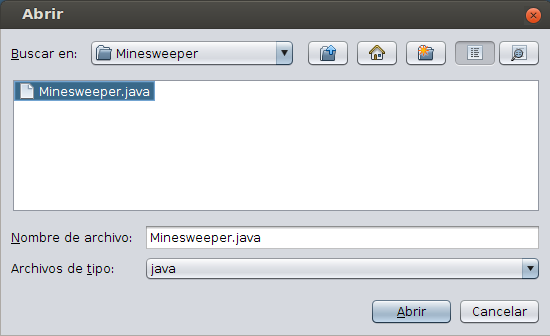
\includegraphics[scale= 0.7]{./cap4/ida_02.png}
}
\caption{Ventana para seleccionar Archivos JAVA}
\label{ida2}
\end{figure}

\vspace{-1em}

\subsection{Lectura de Archivos JAVA}

Cuando se pulsa en el botón \textit{Abrir archivo(s) JAVA}, (Ver Figura \ref{ida1} - Flecha 1), se despliega una ventana para que el usuario elija uno o varios archivos JAVA (Ver Figura \ref{ida2}). 

%Para que IDA funcione correctamente el archivo de entrada JAVA debe cumplir con ciertas validaciones. Una de ellas es, que el código no contenga errores sintácticos (un ejemplo, entre tantos, de error sintáctico es: no colocar punto y coma al final de una sentencia).

Una vez que el usuario elige el/los archivo/s, IDA utiliza un  programa externo llamado JACOBE\footnote[1]{http://www.tiobe.com/jacobe}. Este programa JACOBE, recibe como entrada un archivo JAVA y embellece el código fuente que esta contenido en el. Este embellecimiento se realiza para facilitar la lectura del código al usuario. En la próxima sección se describe el panel que IDA tiene para visualizar el código leído del archivo.

%Si algún archivo de entrada esta vacío o posee algún error sintáctico, JACOBE lo detecta y automáticamente IDA muestra un cartel informando al usuario (ver figura \ref{idaWar1}). 

La herramienta IDA, además realiza un control de los archivos abiertos, impidiendo que se abra el mismo archivo más de una vez. En caso de que esto suceda, se muestra un cartel informando al usuario (Ver Figura \ref{idaWar2}). Este control se realiza por cuestiones de coherencia al momento de analizar los archivos.

%\begin{figure}[t] %[h] para here [b] para bottom [t] para top
%\centerline{%queda centrada mejor la imagen
%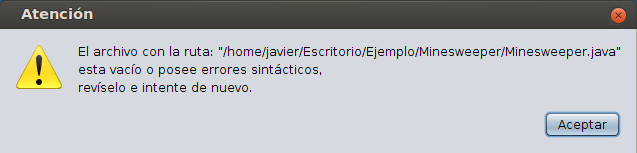
\includegraphics[scale= 0.8]{./cap4/ida_war_01.png}
%}
%\caption{Aviso sobre Archivo JAVA no válido}
%\label{idaWar1}
%\end{figure}

\begin{figure}[t] %[h] para here [b] para bottom [t] para top
\centerline{%queda centrada mejor la imagen
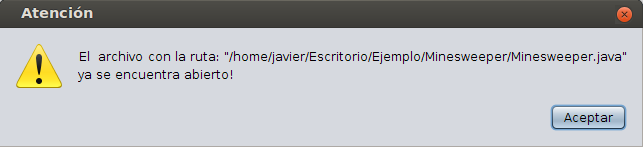
\includegraphics[scale= 0.8]{./cap4/ida_war_02.png}
}
\caption{Aviso sobre Archivo JAVA ya abierto en IDA}
\label{idaWar2}
\end{figure}

\subsection{Panel de Elementos Capturados}

Después que el programa JACOBE embellece el código contenido en el archivo JAVA,
%si estos cumplen con las validaciones descriptas en la sección anterior, 
el mismo se procesa por el AS explicado en secciones previas. Luego que el AS termina sus tareas de extracción de elementos (ids, comentarios y literales), el \textit{Panel de Elementos Capturados} aparece (Ver Figura \ref{ida3}). Este panel en la parte superior posee pestañas, cada pestaña posee un rótulo con el nombre del archivo que está siendo analizado (Ver Figura \ref{ida3} - Flecha 1). Es posible elegir de a varios archivos para analizar, mediante la ventana de selección de archivos (Ver Figura \ref{ida2}), o también se puede ir eligiendo de a un archivo por apertura de esta ventana.  En caso de querer finalizar el análisis de un archivo particular y cerrar la pestaña, se puede pulsar en la cruz ubicada al lado del rótulo de cada pestaña (Ver Figura \ref{ida3} - Flecha 1).

\begin{figure}[t!] %[h] para here [b] para bottom [t] para top
\centerline{%queda centrada mejor la imagen
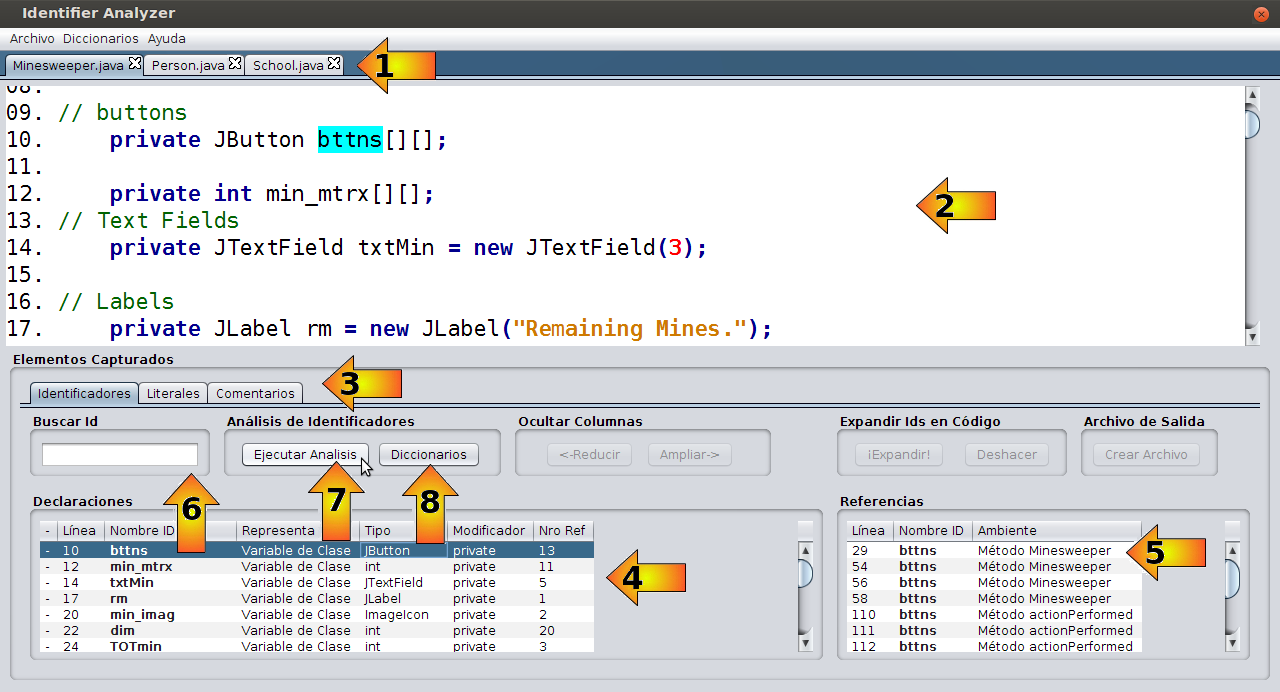
\includegraphics[scale= 0.42]{./cap4/ida_03.png}
}
\caption{Panel de Elementos Capturados}
\label{ida3}
\end{figure}

\begin{figure}[h!] %[h] para here [b] para bottom [t] para top
\centerline{%queda centrada mejor la imagen
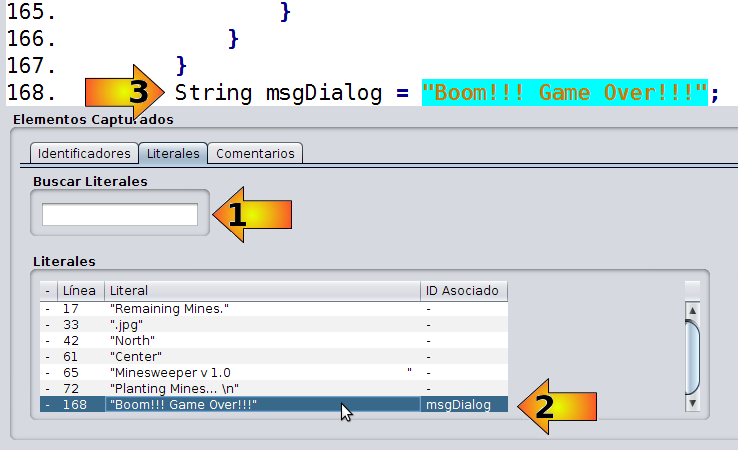
\includegraphics[scale= 0.5]{./cap4/ida_04.png}
}
\caption{Pestaña de Literales Capturados}
\label{ida4}
\end{figure}

Cada pestaña en su interior posee el mismo subpanel que se divide en dos partes principales. La parte superior contiene el código leído y embellecido (por JACOBE) del archivo JAVA (Ver Figura \ref{ida3} - Flecha 2).
%, el código aquí se presenta ya alineado en su formato por JACOBE. duda
La parte inferior, muestra toda la información extraída por el AS referente a ids, literales y comentarios. Estos últimos tres poseen una pestaña cada uno (Ver Figura \ref{ida3} - Flecha 3). Al pulsar sobre cada pestaña, se muestra la información clasificada correspondiente (a ids, literales y comentarios), a continuación se describe como se exhibe esta información.

\noindent \textbf{\\\\Pestaña de Identificadores Capturados\\} 

Al pulsar la \textit{Pestaña de Identificadores} (Ver Figura \ref{ida3} - Flecha 3), se muestra la \textit{Tabla de Declaraciones} (Ver Figura \ref{ida3} - Flecha 4). Esta tabla enumera los ids capturados por el AS y cada columna se corresponde a: el número de línea donde esta declarado el id, el nombre del id, el tipo (int, char, etc.), el modificador (público, privado, protegido), lo que el id representa (variable de clase, constructor, método de clase, etc.).
Esta \textit{Tabla de Declaraciones} si se presiona sobre una fila, inmediatamente se resalta con color en el código ubicado en la parte superior, la declaración del id correspondiente (Ver Figura \ref{ida3} - Flecha 2). 
%Es el mismo comportamiento que tienen las tablas de literales y comentarios explicados anteriormente. 
Cabe destacar que si el usuario lo desea, puede realizar búsquedas en la \textit{Tabla de Declaraciones} por nombre de id; para realizar las estas búsquedas se debe escribir en el cuadro de texto ubicado dentro del recuadro \textit{Buscar Id} (Ver Figura \ref{ida3} - Flecha 5), a medida que se escriba en este cuadro de texto, se irán filtrando los resultados en la \textit{Tabla de Declaraciones}.

\begin{figure}[t] %[h] para here [b] para bottom [t] para top
\centerline{%queda centrada mejor la imagen
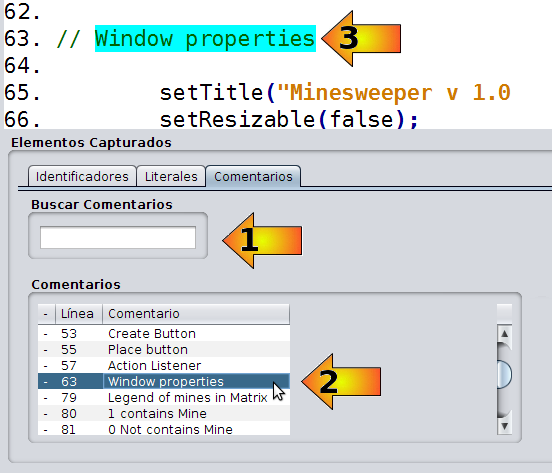
\includegraphics[scale= 0.55]{./cap4/ida_05.png}
}
\caption{Pestaña de Comentarios Capturados}
\label{ida5}
\end{figure}

\noindent \textbf{\\Pestaña de Literales Capturados\\} 

Al pulsar la \textit{Pestaña de Literales} (Ver Figura \ref{ida3} - Flecha 3), se puede apreciar que aparece una \textit{Tabla de Literales} y un práctico buscador en forma de cuadro de texto (Ver Figura \ref{ida4} - Flecha 1 y 2). Esta tabla contiene dos columnas, número de línea del literal y el literal propiamente dicho (Ver Figura \ref{ida4} - Flecha 2).
De manera similar a la que se describió en el párrafo precedente, el buscador filtra los resultados en la \textit{Tabla de Literales} mientras se va escribiendo en el. También al pulsar sobre alguna fila, automáticamente el literal correspondiente se resalta en el código que está ubicado en la parte superior (Ver Figura \ref{ida4} - Flecha 3).

\noindent \textbf{\\Pestaña de Comentarios Capturados\\} 

Al presionar la \textit{Pestaña de Comentarios} (Ver Figura \ref{ida3} - Flecha 3), se visualiza la \textit{Tabla de Comentarios} y un buscador de comentarios en esta tabla (Ver Figura \ref{ida5} - Flecha 1). La \textit{Tabla de Comentarios} posee dos columnas que corresponden, por un lado al comentario y por el otro al número de línea donde se encuentra el comentario dentro del código (Ver Figura \ref{ida5} - Flecha 2). Al igual que se describió en el párrafo anterior, al presionar en una de las filas de la \textit{Tabla de Comentarios} inmediatamente se resalta en el código de la parte superior, la ubicación del comentario seleccionado (Ver Figura \ref{ida5} - Flecha 3).\\

Hasta aquí, solo se ha descripto como IDA exhibe la información útil que fue capturada del código por el AS. A continuación, se explicará como se emplea IDA para analizar los ids. Para ello, se debe pulsar en la \textit{Pestaña de Identificadores} (Ver Figura \ref{ida3} - Flecha 3), luego pulsar en el botón \textit{Ejecutar Análisis} ubicado dentro del cuadro \textit{Análisis de Identificadores} (Ver Figura \ref{ida3} - Flecha 6), al hacerlo se abrirá la \textit{Ventana de Análisis} que será explicada en la próxima sección.

\begin{figure}[h!] %[h] para here [b] para bottom [t] para top
\centerline{%queda centrada mejor la imagen
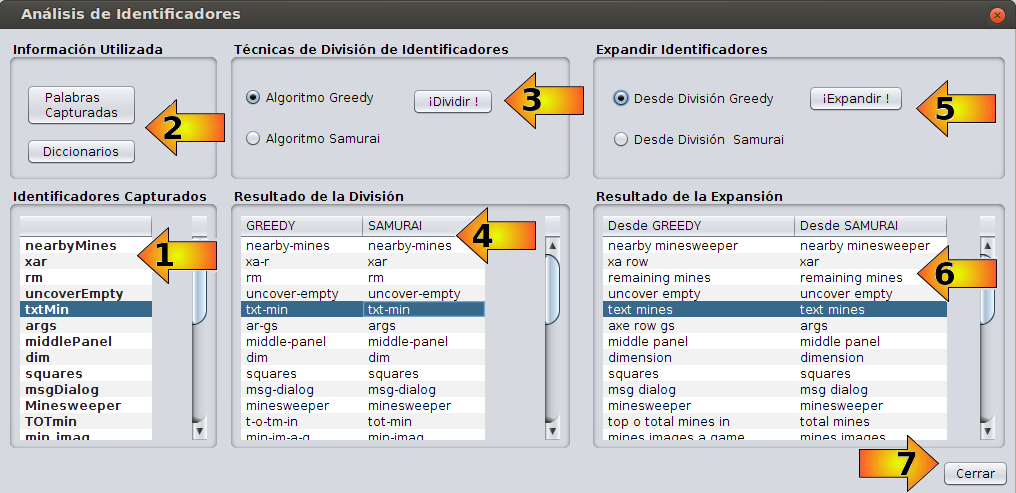
\includegraphics[scale= 0.52]{./cap4/ida_06.png}
}
\caption{Ventana de Análisis}
\label{ida6}
\end{figure}

\subsection{Ventana de Análisis}

La \textit{Ventana de Análisis} (Ver Figura \ref{ida6}) contiene 3 partes principales, (de izquierda a derecha):

\begin{description}

\item[Parte Izquierda:] Posee un listado con los ids capturados, en el cuadro inferior izquierdo (Ver Figura \ref{ida6} - Flecha 1). Arriba de estos se encuentran dos botones \textit{Palabras Capturadas} y \textit{Diccionarios} (Ver Figura \ref{ida6} - Flecha 2), al pulsarlos le brindan información al usuario sobre los datos que se utilizan para ejecutar los algoritmos de análisis, y ambos botones serán explicados con más detalles en la próxima sección.

\item[Parte Central:] Ubicado en la parte central, en el cuadro superior (Ver Figura \ref{ida6} - Flecha 3) se pueden seleccionar los dos algoritmos de división de ids (Greedy y Samurai), el botón \textit{Dividir} del mismo cuadro ejecuta el algoritmo seleccionado. Los resultados obtenidos se muestran en el cuadro central inferior, en una tabla con los resultados. En la Figura \ref{ida6} - Flecha 4 se muestran ambas técnicas (Greedy y Samurai) ya ejecutadas y enumerando los resultados.

\item[Parte Derecha:] Al presionar el botón \textit{Expandir}, situado en el cuadro superior derecho (Ver Figura \ref{ida6} - Flecha 5), ejecuta el algoritmo de expansión básico tomando como entrada los ids divididos desde Greedy o desde Samurai, según haya seleccionado el usuario en este mismo cuadro (Ver Figura \ref{ida6} - Flecha 5). Los resultados obtenidos de las expansiones (desde Greedy y desde Samurai), se muestran en la tabla situada en el cuadro inferior derecho. En la Figura \ref{ida6} - Flecha 6 se pueden apreciar las expansiones realizadas.

\end{description}

\begin{figure}[t] %[h] para here [b] para bottom [t] para top
\centerline{%queda centrada mejor la imagen
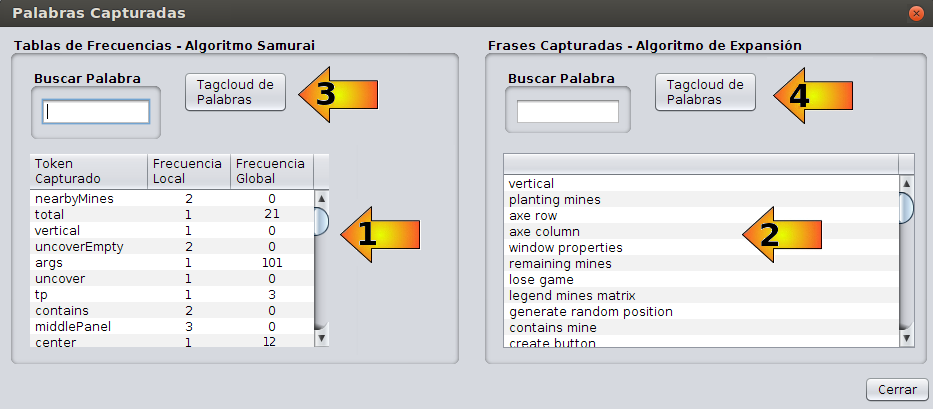
\includegraphics[scale= 0.55]{./cap4/ida_07.png}
}
\caption{Ventana de Palabras Capturadas}
\label{ida7}
\end{figure}

\subsection{Palabras Capturadas y Diccionarios}
\label{sec:panPalDicc}

En la sección anterior, se describieron dos botones \textit{Palabras Capturadas} y \textit{Diccionarios}, ubicados en la \textit{Ventana de Análisis} (Ver Figura \ref{ida6} - Flecha 2). A continuación, se explicarán la función de cada uno de ellos.

\noindent \textbf{\\Ventana de Palabras Capturadas\\} 

Al pulsar el botón \textit{Palabras Capturadas}, se abre una ventana que posee dos cuadros (Ver Figura \ref{ida7}), el cuadro de la izquierda contiene una tabla que muestra las frecuencias correspondiente al Algoritmo Samurai (Ver Figura \ref{ida7} - Flecha 1). Esta tabla tiene tres columnas, en la primera posee palabras\footnote[1]{En este contexto, significa las palabras que están contenidas en literales, comentarios e ids, este último necesita un proceso especial, para más detalles ver Cap. 3 - sección \ref{sec:algSamu}}, las mismas fueron capturadas y procesadas por el AS ANTLR. La segunda columna, contiene la frecuencia local de cada palabra, cabe recordar que la frecuencia local se construye en función de la frecuencia absoluta de aparición de las palabras en el código del archivo actual. La tercera y última columna de la tabla denota la frecuencia global de cada palabra, la misma esta predefinida en la base de datos HSQLDB (Ver sección \ref{sec:bseEmb}).

El cuadro de la derecha, lista en una tabla las frases capturadas (Ver Figura \ref{ida7} - Flecha 2), estas frases se obtienen de los comentarios y los literales strings, el Algoritmo de Expansión es el encargado de utilizarlas (Ver Capítulo 3 - sección \ref{sec:algExpBas}). Este algoritmo las usa, ya que estas frases son posibles candidatas a expandir las abreviaturas en forma de acrónimo que puede contener un id (Ejemplo: \textsf{fs} $\Rightarrow$ \textsf{file system}). También cada una de las palabras por separado, puede ser utilizada para expandir abreviaturas comunes (Ejemplos: \textsf{sys} $\Rightarrow$ \textsf{system}, \textsf{fl} $\Rightarrow$ \textsf{file}).

A modo de agilizar las búsquedas en las tablas descriptas anteriormente (la de frecuencias de Samurai y la de frases), se puede llevar a cabo utilizando los cuadros de texto con rótulo \textit{Buscar Palabra} situados al lado de cada botón \textit{TagCloud de Palabras} (Ver Figura \ref{ida7} - Flechas 3).

\begin{figure}[t] %[h] para here [b] para bottom [t] para top
\centerline{%queda centrada mejor la imagen
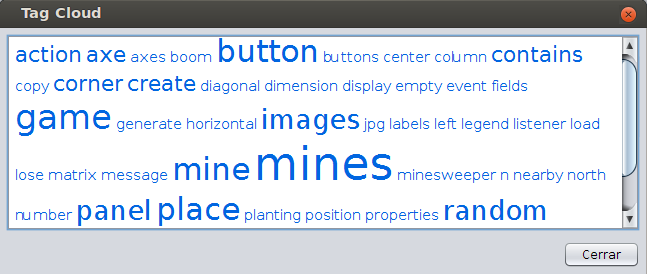
\includegraphics[scale= 0.75]{./cap4/ida_08.png}
}
\caption{Ventana TagCloud (Nube de Etiquetas)}
\label{ida8}
\end{figure}

\noindent \textbf{\\Ventana TagCloud (Nube de Etiquetas)\\} 

Como se puede observar en la Figura \ref{ida7} - Flecha 3, existe un botón con el nombre de \textit{TagCloud de Palabras}, al pulsar sobre este, abre una ventana que contiene una \textit{Nube de Etiquetas} (Ver Figura \ref{ida8}). Esta nube posee palabras y resalta en tamaño más grande aquellas palabras que más frecuencia de aparición tienen (En la Figura \ref{ida8} las palabras \textsf{mine}, \textsf{mines}, \textsf{game} etc. son las que mayor aparición tienen). Para generar esta nube se emplea una librería de JAVA llamada OpenCloud\footnote[1]{http://opencloud.mcavallo.org}.
Esta \textit{Nube de Etiquetas} ayuda a ver con más claridad que palabras son más frecuentes, dado un conjunto de palabras pasado por entrada. 

Para el caso de la \textit{Nube de Etiquetas} correspondiente a la tabla de frecuencias de Samurai (Ver Figura \ref{ida7} - Flecha 3), el tamaño de cada palabra depende de la Frecuencia Local de cada palabra (Ver Figura \ref{ida7} - Flecha 1), mientras más frecuencia tenga la palabra, mayor será el tamaño en la nube. Con esta visualización, se pretende ayudar al usuario a determinar que conceptos son más abundantes en el sistema analizado.

%En el caso de la nube de las frases capturadas (ver figura \ref{ida7} - Flecha 4), el tamaño de las palabras esta dado por el número de apariciones dentro de esta tabla de frases (ver figura \ref{ida7} - Flecha 2).

\begin{figure}[t] %[h] para here [b] para bottom [t] para top
\centerline{%queda centrada mejor la imagen
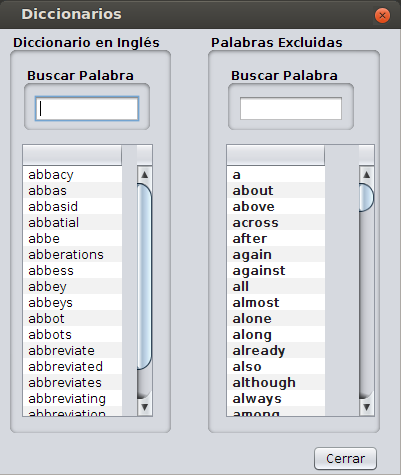
\includegraphics[scale= 0.58]{./cap4/ida_09.png}
}
\caption{Ventana de Diccionarios}
\label{ida9}
\end{figure}

\noindent \textbf{\\Ventana de Diccionarios\\} 

Volviendo a la \textit{Ventana de Análisis} si se pulsa el botón \textit{Diccionarios} (Ver Figura \ref{ida6} - Flecha 2), se abre la \textit{Ventana de Diccionarios} (Ver Figura \ref{ida9}). Esta ventana posee dos tablas, la tabla de la izquierda lista todas las palabras en inglés que tiene el diccionario del comando de Linux \textit{ispell}, esta lista de palabras es utilizada por el Algoritmo Greedy y el Algoritmo Expansión Básica (Ver sección \ref{sec:bseEmb} de este capítulo). La segunda tabla de la derecha enumera las palabras que pertenecen a la stoplist o lista de palabras irrelevantes, también utilizada por los dos algoritmos antedichos. Convenientemente, ambas tablas poseen un buscador por palabras dado que el contenido de cada una es amplio (Ver Figura \ref{ida9}). Esta \textit{Ventana de Diccionarios} puede ser invocada desde otros lugares de la herramienta IDA. Uno de ellos es desde la barra de menú (Ver Figura \ref{ida1} - Flecha 2). Otro sitio donde puede abrirse, es desde el \textit{Panel de Elementos Capturados}, pulsando el botón que esta al lado de \textit{Ejecutar Análisis} (Ver Figura \ref{ida3} - Flecha 7).

Todas las ventanas que fueron descriptas previamente (palabras capturadas, tagcloud, diccionarios), en caso de haber sido abiertas por el usuario, el mismo debe cerrarlas si desea continuar con el proceso de análisis de ids.

\begin{figure}[t!] %[h] para here [b] para bottom [t] para top
\centerline{%queda centrada mejor la imagen
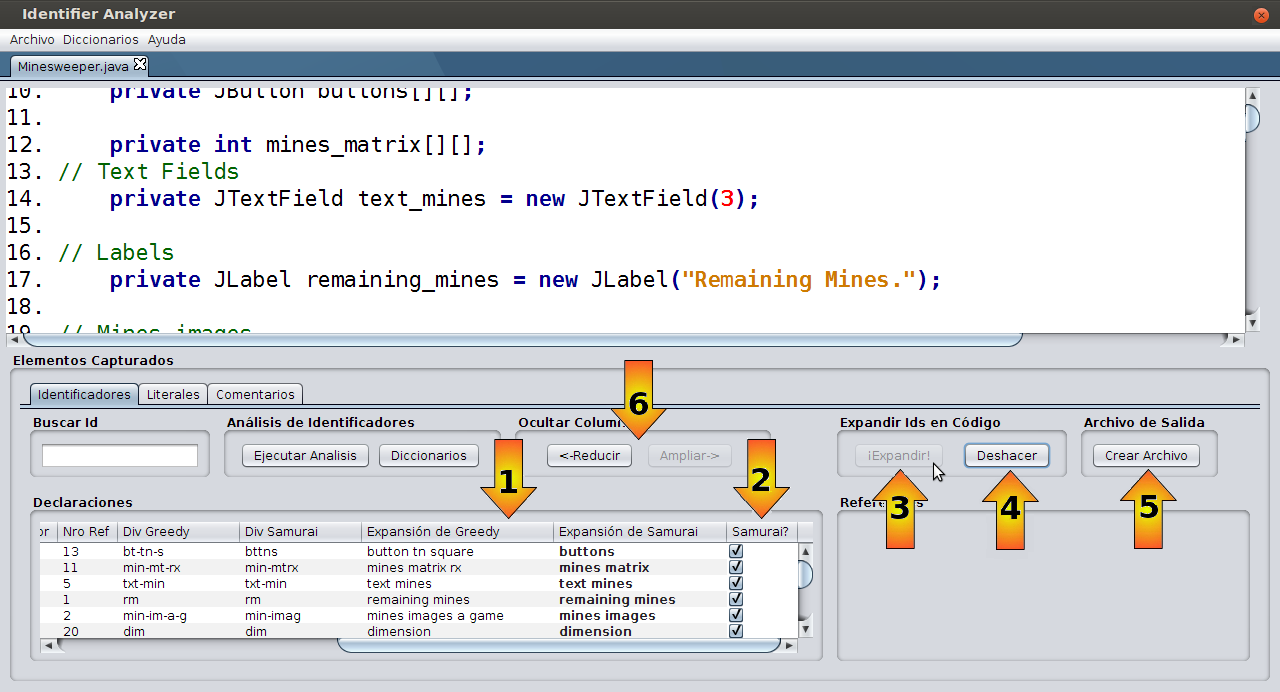
\includegraphics[scale= 0.42]{./cap4/ida_10.png}
}
\caption{Panel de Elementos Capturados}
\label{ida10}
\end{figure}

\begin{figure}[t!] %[h] para here [b] para bottom [t] para top
\centerline{%queda centrada mejor la imagen
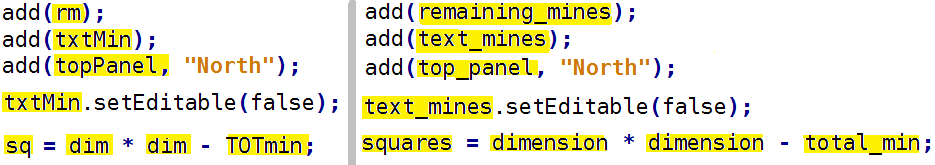
\includegraphics[scale= 0.63]{./cap4/ida_11.png}
}
\caption{Captura del Navegador Web con el Análisis de Ids realizado}
\label{ida11}
\end{figure}

\subsection{Nuevamente al Panel de Elementos Capturados}

Una vez que los ids fueron analizados (Divididos y Expandidos) mediante la \textit{Ventana de Análisis}, la misma debe ser cerrada presionando el botón \textit{Cerrar} (Ver Figura \ref{ida6} - Flecha 7). Esta acción, retorna al \textit{Panel de Elementos Capturados} nuevamente (Ver Figura \ref{ida10}).
Como se puede observar, en la tabla \textit{Declaraciones} que detalla los ids extraídos e información asociada a estos, se le suman nuevas columnas (Ver Figura \ref{ida10} - Flecha 1). Estas nuevas columnas contienen los resultados obtenidos de los algoritmos de división (Greedy, Samurai) y el algoritmo de expansión ejecutados en la \textit{Ventana de Análisis}; las columnas nuevas son: División Greedy, División Samurai, Expansión desde Greedy y Expansión desde Samurai.

Al agregar las columnas nuevas se habilita el cuadro \textit{Ocultar Columnas}. En el se encuentran dos botones \textit{Reducir} y \textit{Ampliar} (Ver Figura \ref{ida10} - Flecha 2). El primero de ellos a modo de facilitar la visualización, oculta las columnas que hay entre los ids y las columnas que contienen el análisis de ids (las columnas que se ocultan son: tipo, modificador, Representa), de esta manera el usuario puede comparar más claramente las distintas divisiones y expansiones de ids. Mientras que el botón \textit{Ampliar} restablece las columnas originales.

%Cuando el usuario termina de seleccionar la mejor expansión de cada id, se procede al cuadro \textit{Expandir Ids en Código}. Este cuadro contiene dos botones, al presionar \textit{Expandir} (ver figura \ref{ida10} - Flecha 3), la herramienta IDA reemplaza los ids del código de acuerdo a lo seleccionado en las casillas de selección en la tabla de \textit{Declaraciones} que fue explicado al principio de esta sección.
%Una vez realizado esto, el código es más comprensivo para el usuario, en la figura \ref{ida11} se puede observar dos trozos de códigos, el de la arriba se observa el código normal, mientras que el de la abajo posee los ids expandidos.
%En caso de querer retrotraer la acción de reemplazo de ids, se puede pulsar en el botón \textit{Deshacer} ubicado también en el cuadro \textit{Expandir Ids en Código} (ver figura \ref{ida10} - Flecha 4) y restablecer el código original.

Luego si el usuario lo decide, puede presionar el botón \textit{Abrir} en el cuadro \textit{Ver Tabla en Navegador} (Ver Figura \ref{ida10} - Flecha 3). Esta acción abre automáticamente el navegador web por defecto del sistema operativo, y mediante una página web en formato html, se muestra una tabla con los resultados obtenidos producto del análisis de ids (Ver Figura \ref{ida11}). De esta manera, el usuario puede visualizar más claramente el análisis realizado, permitiendo también imprimir los resultados en papel (mediante el navegador web), si el usuario lo desea.

Dando como finalizado el proceso necesario que debe realizar el usuario para analizar los ids con la herramienta IDA, en el próximo capítulo se describen algunos casos de estudio que demuestran la importancia de haber construido IDA.

